\documentclass{article}
\usepackage[T1]{fontenc}
\usepackage{lmodern}
\usepackage{graphicx}
\usepackage{amsmath,amssymb}
\usepackage[a4paper,margin=2cm]{geometry}
\usepackage[absolute,overlay]{textpos}
\setlength{\TPHorizModule}{1mm}
\setlength{\TPVertModule}{1mm}
\usepackage[indonesian]{babel}
\usepackage{hyperref}
\setlength{\emergencystretch}{2em}
% unit: Halaman 43

\begin{document}

% === Halaman 43 (llm) ===

\vspace{190.08mm}

Pada citra 24-bit (\textit{real image}), 1 pixel = 24 bit, terdiri dari komponen RGB (Red-Green-Blue)

% deskripsi: Ilustrasi representasi warna sebuah pixel pada citra 24-bit menggunakan model RGB, menunjukkan sebuah pixel dari foto Taj Mahal yang dipetakan ke rangkaian bit biner yang dibagi menjadi tiga bagian: Red (merah), Green (hijau), dan Blue (biru).
% bbox normalisasi: [0.1410, 0.2860, 0.9060, 0.9260]
\begin{textblock*}{160.65mm}(29.61mm,84.94mm)
\noindent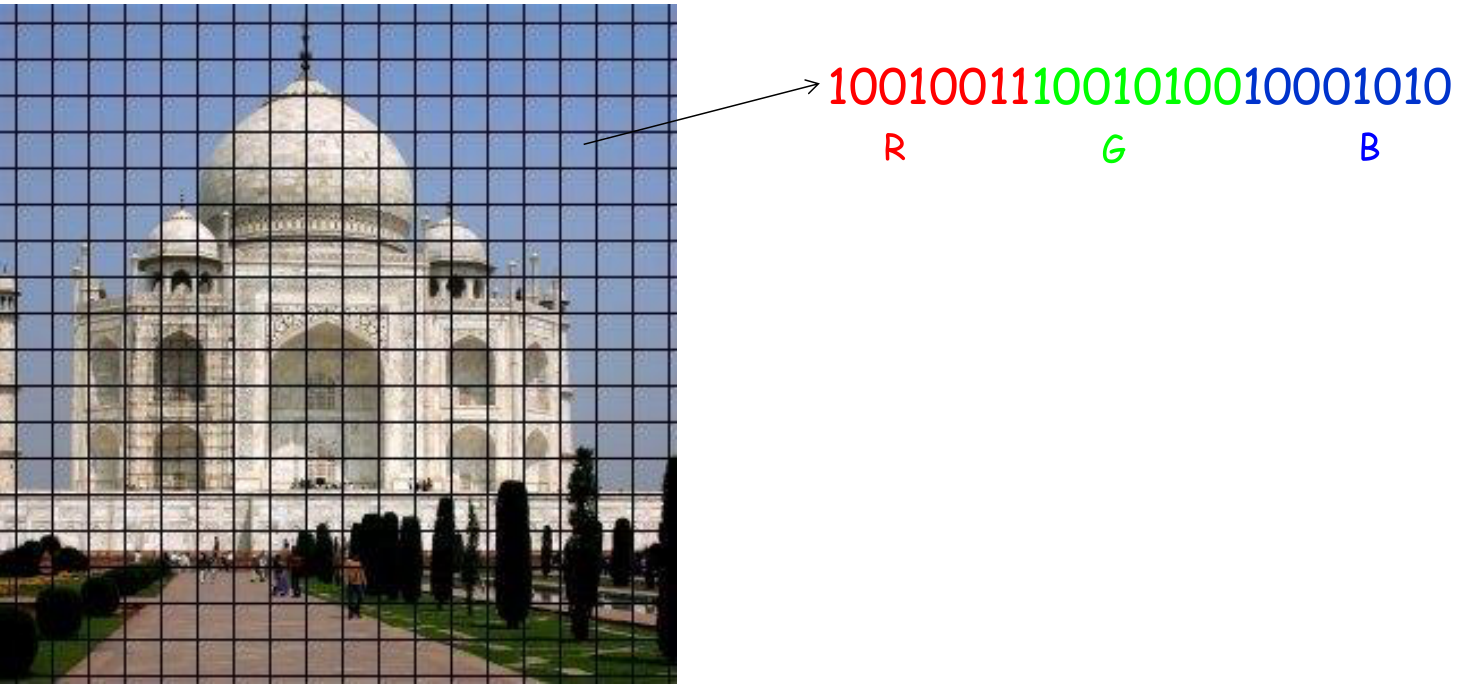
\includegraphics[width=160.65mm,height=190.08mm]{../../images/llm/page_043_img_01.png}%
\end{textblock*}

\end{document}
